%!TEX root = ../dissertation.tex
\begin{savequote}[75mm]
Nulla facilisi. In vel sem. Morbi id urna in diam dignissim feugiat. Proin molestie tortor eu velit. Aliquam erat volutpat. Nullam ultrices, diam tempus vulputate egestas, eros pede varius leo.
\qauthor{Quoteauthor Lastname}
\end{savequote}

\chapter{Evaluation}


\newthought{Realistic evaluation is a vital part of a good project report.}
For software projects, describe the evaluation methods used; discuss reliability
and usability of the end-product; where appropriate, obtain client views. To
what extent have the specified objectives of the project been met? How
successful and appropriate was the methodology adopted? Wherever possible,
support your views with evidence.
For research projects, discuss the merit of research methods/approaches
employed; if you didn’t already do so in your Deliverable chapter, compare the
merit of your methods, where applicable, with other possible alternatives,
Consider the limitations of the research, including limitations on the
generalisability of the results obtained/recommendations made/guidelines
suggested – providing sound argument for these limitations. Outline the
lessons learned as a result of the research and discuss scope and directions for
future research.
Computer Science, SEAS, Aston University – 5 – DC3010 Instructions 2016/17
This section should be answering the question: “How do I know if the
deliverable met its goals?”
Include an assessment of the business value of the deliverable.

\section{Extending the impact}
With one of my manifest items being ``Make an impact over getting a good
grade" I was looking for opportunities throughout the project to extend this.
Below I have documented some additional deliverables which came out of the
project as direct side effects of the work done.

\subsection{Markdown/React Documentation Framework}
\subsection{Colour Contrast Tool}
Whilst I was creating the A11Y Guide I was asked to experiment with an
upcoming piece of technology. ``CSS in JS" \citep{CSSInJS}. The industry has been moving
towards `component driven' development \citep{CDD} through the entrance of
Angular
and ReactJS; CSS in JS is the last step in all code relating to a
component being co-located in a single file. Myself like others had had
significant reservations \citep{AgainstCssInJs} about the performance and portability of
such an idea. However, working for a technology consultancy firm we are
advised to form an opinion on any impacting changes within our retrospective
spaces.

Having done research into colour contrast tools as part of the A11Y Guide I
identified a gap for a ``modern", user focussed tool. Most current tools
require submission to a server and lack demonstrations
of what the two colours look like when used together \cite*{JuicyStudio}. All
of them satisfied a relatievly simple set of requirements:
\begin{itemize}
\item Report the colour contrast level between two distinct colours
\item Report whether the colours contrast level of such colours satisfies the
 WCAG guidelines for the ``wanted" text size.
\end{itemize}

Using Moqups \citep{Moqups} I quickly put together a quick design using
their colour schemes and fonts See \ref{fig:colour_contrast_1}. To test out
``CSS in JS" I wanted to use `Styled Components' a ReactJS implementation
written by \cite*{StyledComponents} which has gained real traction. ``Create
React App" was again used to speed up the development process. This was
only an `experiment' and thus to be completed quickly, testing was reduced to
cover only the core logic for calculating colour contrast.

\begin{figure}[H]
\centering
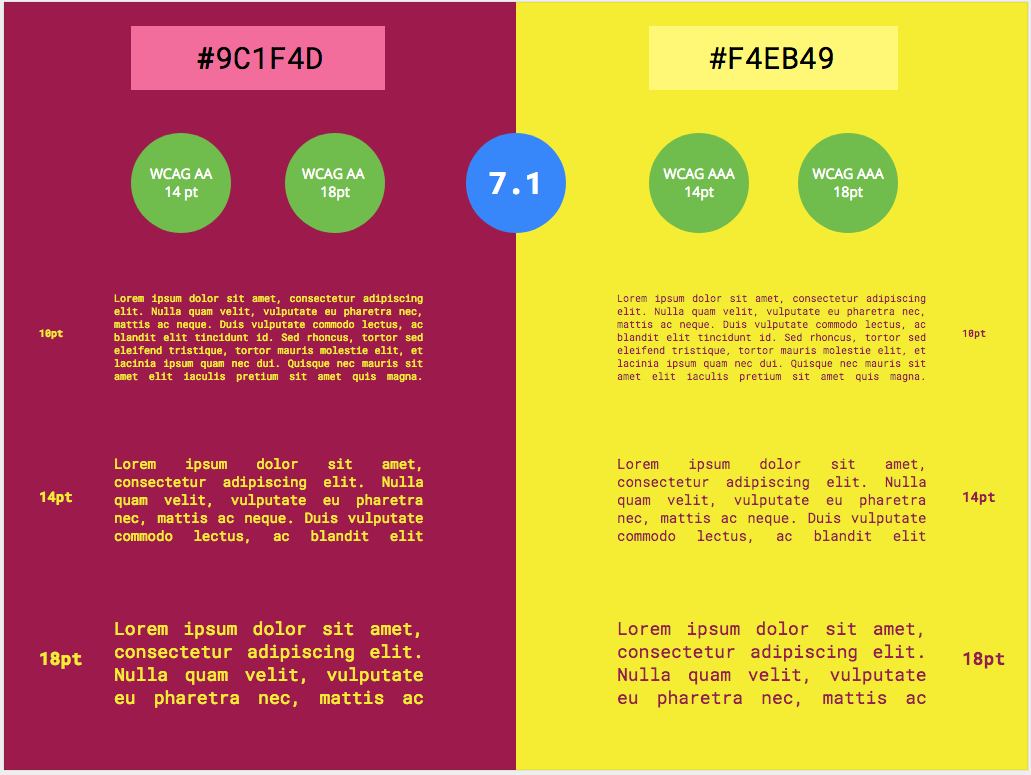
\includegraphics[width=0.65\textwidth]{figures/colour_contrast_1}
\captionsetup{justification=centering}
\caption{Design for Colour Contrast tool
\label{fig:colour_contrast_1}}
\end{figure}

The `Happy Day' user journey would be:
\begin{itemize}
\item User enters first colour in input field (Can paste)
\item User enters second colour in input field
\item On a valid colour entered. Both are displayed as background and
foreground; the value of colour contrast is displayed; and the contrast
levels WCAG appropriateness is displayed in the circles. Green for success, Red
for failure.
\end{itemize}

In the error scenario of a user entering an invalid colour, the background
colours would remain the same and the input field would have a `red'
background and border to signify an error.

This was deployed through github pages to \url{https://colour-contrast.github.io/}
and was tweeted about by myself and
subsequently the creator of 'styled-components'. In the month
the tool has been live it has gained \textasciitilde450 views across most
countries. It receives \textasciitilde3-4 views a day now.

\begin{figure}[H]
\centering
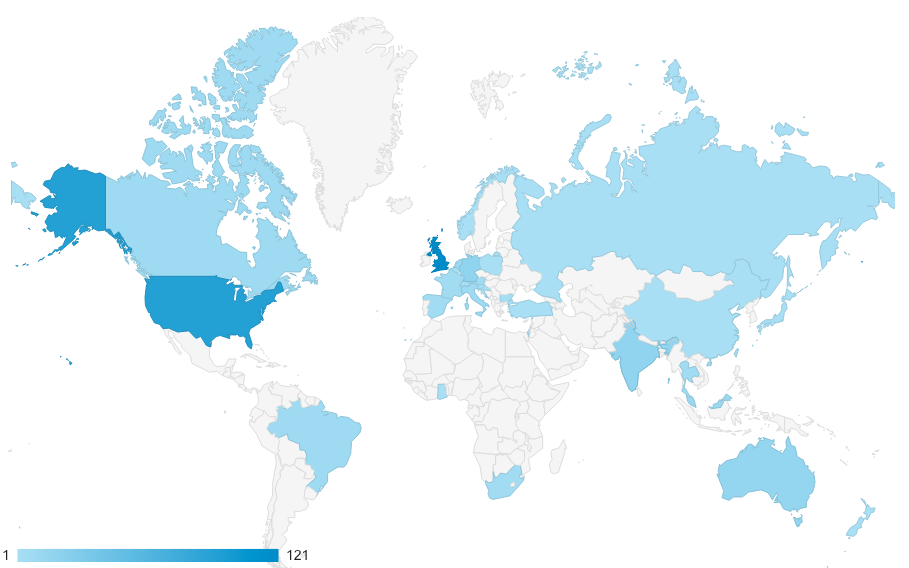
\includegraphics[width=0.65\textwidth]{figures/colour_contrast_analytics}
\captionsetup{justification=centering}
\caption{Google Analytics location based viewing statistics
\label{fig:colour_contrast_analytics}}
\end{figure}


% TODO - Maybe discuss impact here.. or evaludation..

